%Modelo Descentralizado- Especificar como a equipa vai funcionar.
%Conclusão do COCOMO

%formatação do documento e tipo do documento
\documentclass[12pt, a4paper, twoside]{report} %inicio do doc

%pacotes de extensões
\usepackage[portuges]{babel} %pkg da lingua portugues
\usepackage[latin1,utf8]{inputenc} %pkg da lingua portugues
\usepackage{verbatim} %pkg para escrever sem formataçao
\usepackage{color} %usar cores nas letras
\usepackage{graphicx} %usar imagens no doc
\usepackage[table,xcdraw]{xcolor}
\usepackage{makeidx}
\usepackage{anysize} % para formatar o tamanho do documento
\usepackage{multirow}
\usepackage{mathtools}
\usepackage{wrapfig}
\usepackage{footnote}

\marginsize{3.17cm}{3.17cm}{2.54cm}{2.54cm}

%fazer índice
\makeindex

\begin{document}

\title{%
	\textbf{Planeamento e Gestão de Projecto}\\ 
	\large Relatório Fase 2
}

\author{%
Alexandre Machado, nº 43551 \\
Nuno Silva, nº 44285 \\
Francisco Pires, nº 44314 \\
}

\date{\today}
\maketitle
\tableofcontents

%--------------------------------------------------------------------------------------------- Feito
\chapter{Introdução}

\textit{Foram feitas alterações nas partes entregues na primeira e segunda fase} \\


Este projecto tem como objectivo o desenvolvimento e a implementação de um Sistema de Informação (SI), dirigido aos utentes do Serviço Nacional de Saúde (SNS). 
Este relatório vai abordar a analise dos requisitos, o planeamento e por ultimo a arquitetura que vai ser necessária para a realização deste projecto.


O objectivo final vai ser construir um SI mais eficaz e seguro, que agregue mais funcionalidades que o actual. Para isso, foi feito um levantamento extensivo das funcionalidade que podem ser introduzidas no  Portal de Utente, sem que estas sejam inconsistentes com os restantes serviços disponibilizados pelo SNS. Para alem disso, foi também feita um levantamento das melhores tecnologias a utilizar neste tipo de projectos, para poder cumprir todos os requisitos não funcionais que vão ser referidos mais a frente no relatório.

Pretendemos também com a realização do planeamento e do SI familiarizar-nos com as técnicas e tecnologias a serem utilizadas no mercado de trabalho.

%--------------------------------------------------------------------------------------------- Feito

\chapter{Análise de requisitos}

\section{Requisitos funcionais e não funcionais}

\subsection{Requisitos funcionais}

De acordo com os objectivos definidos para este projecto, selecionamos as seguintes funcionalidades que o utilizador terá disponíveis neste SI.

\begin{itemize}

\item Registo de contactos e dados pessoais
	\begin{itemize}
	\item Nº Cartão de Cidadão, Nº Utente de Saúde, Nº telefone, Nº Identificação Fiscal, Email
	\end{itemize}
\item Definir agregado familiar
	\begin{itemize}
	\item Pai, mãe, filhos, irmãos, etc...
	\end{itemize} 
\item Identificação de cuidador familiar 
\item Registo de informação pessoal relevante
	\begin{itemize}
	\item Testamento Vital, Contados de emergência
	\end{itemize}
\item Registo de indicadores básicos de saúde
	\begin{itemize}
	\item Medicação, alergias, diagnósticos, cirurgias, vacinação, doenças raras
	\end{itemize}
\item Registo de exames complementares de diagnóstico
	\begin{itemize}
	\item Todo o tipo de exames(documentos relevantes) que o utente faça podem ser guardados no portal pelo próprio
	\end{itemize}
\item Consulta de registos clínicos
\item Pedido de prescrição de medicação crónica
	\begin{itemize}
	\item No caso da medicação crónica, o portal pode gerar receitas automaticamente mediante as instruções do medico.
	\end{itemize}
\item Marcação de consultas
\item Inscrição e consulta das listas para cirurgia (eSIGIC)
\item Definir estado no Registo Nacional de Não Dadores (RENNDA)
\item Pesquisa de serviços médicos (directório)
	\begin{itemize}
	\item Poder pesquisar serviços médicos por área
	\end{itemize}
\item Pedido de mudança de médico de família
\item Pedido de isenção de taxas moderadoras

\end{itemize}

%--------------------------------------------------------------------------------------------- Feito

\subsection{Requisitos não funcionais}

Para execução das funcionalidades neste SI, será necessário assegurar os requisitos não funcionais que listamos de seguida.

\begin{itemize}
\item Confidencialidade dos dados
	\begin{itemize}
	\item Alguns dados médicos que o utente introduz na plataforma só vão poder ser acedidos pelo seu médico mediante autorização do utente.
	\end{itemize}
\item Segurança dos dados e dos acessos
	\begin{itemize}
	\item O acesso aos dados de um utilizador especifico vai somente ser permitido a esse utilizador e aos seus médicos. Para aceder a esses dados deve-se:
		\begin{itemize}
		\item Como utilizador - autenticar a sua conta
		\item Como médico - autenticar a sua conta e esperar que o sistema automaticamente dê as devidas permissões de acesso aos dados do utilizador.
		\end{itemize}
	\end{itemize}
\item Garantia de disponibilidade
	\begin{itemize}
	\item Garantir que a plataforma está sempre acessível online (24/7).
	\end{itemize}
\item Escalável e modular
	\begin{itemize}
	\item Capacidade de poder aumentar a capacidade de servir um maior numero de clientes, iniciando paralelamente mais instâncias do servidor de aplicação e de \textit{web}.
	\end{itemize}
\item Tempo de resposta
	\begin{itemize}
	\item A plataforma terá um tempo de resposta inferior a 500ms.
	\end{itemize}
\item Assegurar o cumprimentos das normas legais do SNS
\item Resolução de conflitos
	\begin{itemize}
	\item Garantir que a informação que o utente e o médico introduzem não divergem, fazendo \textit{merge} de todos os dados introduzidos e pedir aos utilizadores para confirmarem as alterações feitas.
	\end{itemize}
\item Persistência, sincronização dos dados e Disponibilidade
	\begin{itemize}
	\item A informação guardada nos vários servidores vai ser distribuída por várias instâncias. Estas instâncias vão ser sincronizados automaticamente para não haver falhas de persistência e de sincronização, e para alem disso, vai permitir uma rápida recuperação para o SI poder tolerar falhas de hardware.
	\end{itemize}
\item Notificações e alertas de acontecimentos do utilizador
\begin{itemize}
\item Estas serão enviadas para o utente ou o medico via email ou telemóvel
\end{itemize}
\item \textit {Responsive Web Design}
\begin{itemize}
\item Garantir que o site pode ser acedido por várias tipos de dispositivos (\textit{e.x: tablets, smartphones, etc})
\end{itemize}
\end{itemize}

\clearpage

%--------------------------------------------------------------------------------------------- Feito

\section{Modelo de casos de uso}

\subsection{Casos de uso textuais}

\textbf{Consultar registos clínicos}
\\
\\
Ator Principal: Utilizador.\\
Interesses: O utilizador pretende consultar os seus registos clínicos.\\
\\
Pré-condições: O utilizador está registado na plataforma.\\
Pós-condições: O utilizador consiga visualizar os seus registos clínicos com sucesso.\\
\\
Cenário principal de sucesso: 
	\begin{enumerate}
	\item O utilizador indica que quer consultar os seus registos clínicos.
	\item O sistema mostra todos os registos existentes sobre o utilizador.
	\end{enumerate}

\noindent Cenários alternativos:
	\begin{enumerate}
	\item [2.b.] O utilizador não tem informação registada nos seus registos.
	\item [3.b.] O sistema notifica o utilizador que ainda não registou os seus registos médicos.
	\item [4.b.] O sistema dá oportunidade para o utilizador completar os seus registos médicos.
	\item [5.b.] O utilizador escreve os seus registos médicos.
	\end{enumerate}

\noindent\textbf{Marcar cirurgias}
\\
\\
Ator Principal: Utilizador.\\
Interesses: O utilizador pretende marcar uma cirurgia.\\
\\
Pré-condições: Utilizador está autorizado a marcar a cirurgia por um elemento medico.\\
Pós-condições: Utilizador consegue marcar uma cirurgia numa certa data com sucesso.\\
\\
Cenário principal de sucesso:
	\begin{enumerate}
	\item O utilizador indica que quer marcar uma cirurgia.
	\item O sistema notifica ao utilizador que foi autorizado a marcar uma cirurgia de um certo tipo.
	\item O sistema mostra as datas disponíveis pelo sistema para a marcação.
	\item O utilizador marca a cirurgia numa das datas disponíveis.
	\end{enumerate}

\noindent Cenários alternativos:
	\begin{enumerate}
	\item [2.b.] O utilizador não tem autorização para marcar a cirurgia.
	\item [3.b.] O sistema informa o utilizador que este não tem autorização para marcar a cirurgia pretendida.
	\item [4.b.] O sistema informa o utilizador para se dirigir a um posto medico para receber a tal autorização.
	\end{enumerate}

\noindent\textbf{Registar exames}
\\
\\
Ator Principal: Utilizador.\\
Interesses: Utilizador pretende marcar um exame.\\
\\
Pré-condições: Utilizador está autorizado a marcar o exame por parte de um elemento médico.\\
Pós-condições: Utilizador consegue marcar um exame numa certa data com sucesso.\\
\\
Cenário principal de sucesso: 
	\begin{enumerate}
	\item O utilizador indica que quer marcar uma exame.
	\item O sistema notifica ao utilizador que foi autorizado a marcar um exame de um certo tipo.
	\item O sistema mostra as datas disponíveis pelo sistema para a marcação.
	\item O utilizador marca o exame numa das datas disponíveis.
	\end{enumerate}

\noindent Cenários alternativos:
	\begin{enumerate}
	\item [2.b.] O utilizador não tem autorização para marcar o exame.
	\item [3.b.] O sistema informa o utilizador que este não tem autorização para marcar o exame pretendido.
	\item [4.b.] O sistema informa o utilizador para se dirigir a um posto medico para receber a tal autorização.
	\end{enumerate}

\noindent\textbf{Pedir medicamentos}
\\
\\
Ator Principal: Utilizador.\\
Interesses: O utilizador pretende renovar os seus medicamentos.\\
\\
Pré-condições: A receita é renovável e está dentro da data limite desta (seis meses).\\
Pré-condições: A receita é passada pelo medico de família do utilizador.\\
Pós-condições: O utilizador consegue renovar a sua dose do medicamento em questão.\\
\\
Cenário principal de sucesso:
	\begin{enumerate}
	\item O utilizador navega até à pagina de renovações de medicação.
	\item O sistema informa que utilizador têm uma receita renovável.
	\item O utilizador escolhe a receita pretendida.
	\item O utilizador imprime a receita para levar à farmácia.
	\end{enumerate}

\noindent Cenários alternativos:
	\begin{enumerate}
	\item [2.b.] O sistema informa o utilizador que este tem uma receita prescrita por um medico de família.
	\item [3.b.] O sistema informa o utilizador que para renovar a medicação desta receita, o utilizador têm que se dirigir ao medico em questão para uma nova consulta.
	\item [2.c.] O sistema informa o utilizador que este não têm nenhuma medicação que possa ser renovada.
	\end{enumerate}

\noindent\textbf{Marcar consulta}
\\
\\
Ator Principal: Utilizador.\\
Interesses: O utilizador pretende marcar uma consulta com um profissional de saúde.\\
\\
Pré-condições: Ter medico de família e estar registado no portal.\\
Pós-condições: O utilizador consegue marcar uma consulta com um profissional de saúde com sucesso.\\
\\
Cenário principal de sucesso:
	\begin{enumerate}
	\item O utilizador navega até à secção de marcação de consultas.
	\item O sistema verifica se o utilizador têm um medico de família.
	\item O sistema mostra datas disponíveis para o medico de família do utilizador
	\item O utilizador marca uma consulta conforme os horários mostrados.
	\item O sistema informa o utilizador que a sua consulta está em estado de aprovação por parte do medico.
	\item O sistema informa o medico que um utilizador quer marcar uma consulta para aquela data.
	\item O medico escolhe aceitar ou não aceitar a consulta.
		\begin{enumerate}
		\item [8.a.] O utilizador recebe uma notificação com a aprovação da consulta feita pelo medico.
		\item [8.b.] O utilizador recebe uma notificação a dizer que o medico não aceita a consulta marcada.
		\end{enumerate}
	\end{enumerate}

\noindent Cenários alternativos:
	\begin{enumerate}
	\item [3.b.] Se não têm medico de família:
	\item [4.b.] O sistema mostra as datas para a marcação de uma consulta externa.
	\item [5.b.] O utilizador marca uma consulta para um medico disponível no centro de saúde mais próximo.
	\item [6.b.] O sistema informa o utilizador que a sua consulta está em fase de aprovação pelo medico escolhido.
	\item [7.b.] O sistema informa o medico que um utilizador quer marcar uma consulta para aquela data.
	\item [8.b.] O medico escolhe aceitar ou não aceitar a consulta.
	\item [9.b.a.] O utilizador recebe uma notificação com a aprovação da consulta feita pelo medico.
	\item [9.b.b.] O utilizador recebe uma notificação a dizer que o medico não aceita a consulta marcada.
	\end{enumerate}

%--------------------------------------------------------------------------------------------- Feito (REVER)

\subsection{Diagrama modelos de uso}

Em anexo, o ficheiro \textit{DiagramaModelosDeUso.png} encontra-se o diagrama representado os Modelos de Uso do Utilizador e do Médico.

\section{Esboço das interfaces}

Em anexo, na pasta \textit{Interface} encontra-se vários \textit{*.png} com os vários esboços das interfaces.

\section{Modelo de dados e requisitos detalhados}

Em anexo, o ficheiro \textit{ModeloDeDados.png} encontra-se o modelo de dados.

%--------------------------------------------------------------------------------------------- FAZER

\chapter{Planeamento}

\section{Recursos}

\subsection{Recursos Humanos}

Os recursos humanos para o projecto incluem seis alunos de Tecnologias de Informação (LTI), sendo que os três alunos não presentes neste relatório pertencem ao grupo 003. 
No final da cadeira de Planeamento e Gestão do Projecto (PGP), os dois grupos irão juntar-se e trabalhar em conjunto nas cadeiras de Projecto Tecnologias de Informação (PTI) e Projecto Tecnologias de Redes (PTR). A duração total do projecto será de sete meses, sendo três meses e meio dedicados ao planeamento (PGP).

\subsection{Disponibilidade}

A disponibilidade dos alunos é conforme apresentada na seguinte tabela:

\begin{table}[h]
\centering
\begin{tabular}{|l|c c|}
\hline
\multirow{2}{*}{} & \multicolumn{2}{c|}{Disponibilidade} \\ \cline{2-3} 
						& 1ºSemestre        & 2ºSemestre       \\ \hline
Pedro Neves       		& 20\%              & 40\%             \\ \hline
Rita Capela       		& 20\%              & 28,6\%           \\ \hline
Tiago Maurício    		& 20\%              & 28,6\%           \\ \hline
Francisco Pires   		& 20\%              & 33,3\%           \\ \hline
Alexandre Machado 		& 20\%              & 28,6\%           \\ \hline
Nuno Silva\footnotemark	& 10\%              & *                \\ \hline
\end{tabular}
\caption{Tabela de Disponibilidade}
\label{disponibilidade}
\end{table}

\footnotetext{ O aluno em questão encontra-se a trabalhar em \textit{part-time}, pelo que no primeiro semestre tem menos disponibilidade. Não sendo possível prever, por agora, a sua disponibilidade no segundo semestre, foi decidido não ser calculada.}

\clearpage

%--------------------------------------------------------------------------------------------- Feito

\subsection{Organização da equipa}

A organização dos membros envolvidos vai ser feita em três grupos, utilizando um modelo horizontal (democrática e descentralizada).
Um grupo para PTR, um para PTI, e um ultimo grupo para os \textit {"elementos moveis"}. 
Estes alunos vão contribuir em conjunto para o trabalho de ambas as cadeiras, e ao mesmo tempo, gerir o funcionamento e as decisões dos grupos.

\begin{itemize}
\item Grupo PTR
\begin{itemize}
	\item Francisco Pires
	\item Nuno Silva
\end{itemize}
\item Grupo PTI
\begin{itemize}
	\item Tiago Maurício
	\item Rita Capela
\end{itemize}
\item \textit{Elementos Moveis}
\begin{itemize}
	\item Alexandre Machado
	\item Pedro Neves
\end{itemize}
\end{itemize}

\subsection{Tabela de competências}

\begin{table}[h]
\centering
\begin{tabular}{|l|ccccccccccccccc|}
\hline
                  & 1 & 2 & 3 & 4 & 5 & 6 & 7 & 8 & 9 & 10 & 11 & 12 & 13 & 14 & 15 \\ \hline
Pedro Neves       & 3 & 4 & 3 & 2 & 4 & 4 & 1 & 4 & 3 & 2  & 4  & 4  & 4  & 4  & 3  \\ \hline
Rita Capela       & 3 & 2 & 4 & 4 & 3 & 4 & 4 & 4 & 4 & 3  & 1  & 4  & 4  & 3  & 4  \\ \hline
Tiago Maurício    & 3 & 4 & 4 & 3 & 4 & 4 & 2 & 3 & 3 & 2  & 3  & 4  & 4  & 4  & 4  \\ \hline
Francisco Pires   & 2 & 3 & 4 & 3 & 4 & 3 & 3 & 4 & 4 & 2  & 3  & 4  & 4  & 4  & 3  \\ \hline
Alexandre Machado & 2 & 4 & 4 & 4 & 4 & 4 & 3 & 4 & 4 & 3  & 3  & 3  & 4  & 3  & 4  \\ \hline
Nuno Silva        & 2 & 4 & 4 & 4 & 4 & 4 & 3 & 3 & 3 & 2  & 4  & 4  & 4  & 4  & 3  \\ \hline
\end{tabular}
\caption{Tabela de Competências}
\label{competencias1}
\end{table}

\begin{enumerate}
\item PHP
\item Java
\item HTML
\item CSS
\item Python
\item MySQL
\item Interface
\item Gestão
\item Analise
\item Desenho
\item Testes
\item Comunicação
\item Trabalho em equipa
\item Trabalho sobre pressão
\item Capacidade em cumprir prazos
\end{enumerate}

\subsection{Justificações}

A utilização de dois gestores num único projecto é uma organização de equipa excecional. Esta decisão foi tomada tendo em conta as características únicas deste grupo. Os membros de PTI e PTR foram escolhidos baseados nas suas competências técnicas, sendo que isto criou um conflito, pois os dois restantes membros consideram ter ambos competências técnicas equivalentes nas duas cadeiras. Isto, a juntar ao facto destes dois membros serem bastante superiores em termos de gestão de trabalho, levou-nos a tomar esta decisão incomum. Em termos práticos, estes dois elementos vão gerir equipas diferentes, só tendo de tomar decisões juntos quando influenciar todos os elementos ou projecto num todo.

\clearpage

\subsection{Recursos de hardware e de software}

Alguns destes pontos vão ser mais detalhados no capitulo 4.

\subsubsection{Recursos de software}

\begin{itemize}
\item Sistema Operativo: Ubuntu Server 14.4.
\item Servidor Web: WildFly (existe a possibilidade de usar outro servidor baseado em Apache).
\item Uma base de dados relacional MySQL.
\item Java, versão 8 (utilizando as API de JEE para desenvolver o servidor aplicacional).
\item IDE de Java (IntelliJ IDEA ou Eclipse)
\end{itemize}

\subsubsection{Recursos de hardware}
\begin{itemize}
\item Servidores da Amazon (ou outro servidor \textit{cloud-based}) 
\item Computadores da ADMIN-FCUL para testes e servidores locais
\end{itemize}

\clearpage

%--------------------------------------------------------------------------------------------- ACABAR

\section{Estimação}

Para a realização da tabela relativa aos dados históricos, foram escolhidas as cadeiras em que a matéria dos projectos se encaixa no âmbito do projecto.

\begin{table}[h]
\centering
\begin{tabular}{|l|c c c c c|}
\hline
				  & AD        & ASW       & ITW     & ADS     & SO      \\ \hline
Alexandre Machado & 1002/160h & 2576/160h & 756/72h & 454/18h & 560/42h \\ \hline
Francisco Pires   & 1002/160h & NA        & 687/5h  & NA      & 775/50h \\ \hline
Nuno Silva        & 942/150h  & NA        & 542/10h & 500/35h & 700/60h\\ \hline
\end{tabular}
\caption{ Dados Históricos (\textit{Lines of Code} e horas).}
\label{my-label}
\end{table}

\subsection{Esforço disponível}

\begin{itemize}

\item 1º semestre (duração: 3,5 meses)
\begin{equation}
20+20+20+20+20+10 = 110 \ (1,1 \ pessoas)
\end{equation}
\begin{equation}
E = 1,1 \ . \ 3,5 = 3,85 \ PM
\end{equation}
\item 2º semestre (duração: 3,5 meses)
\begin{equation}
40+28,6+28,6+33,3+28,6 = 188 \ (1,88 \ pessoas)\\
\end{equation}
\begin{equation}
\ E = 1,88 \ . \ 3,5 = 6, 58 \ PM
\end{equation}
\end{itemize}

\subsection{Linhas de código}

As linhas de código previstas para o projecto são conforme apresentadas na seguinte tabela:

\begin{savenotes}
\begin{table}[h]
\centering
\begin{tabular}{|l|c c c c|}
\hline
										& Optimista & Provável & Pessimista & \textbf{Final} \\ \hline
Criar a Base de Dados  					& 50        & 120      & 200        & 123   		 \\ \hline
Configurar \textit{HTTP Server} 		& 5         & 20       & 50         & 25    		 \\ \hline
Ligação à Base de Dados \footnote{Linhas a não serem consideradas usando a linguagem \textit{Java}.}
										& 5         & 10       & 20         & 12    		 \\ \hline
Segurança              					& 200       & 300      & 350        & 283   		 \\ \hline
Sistema Distribuído\footnotemark	    & 2000      & 3750     & 5000       & 3583   		 \\ \hline
\textit{Views}            				& 1000      & 1500     & 2500       & 1600  		 \\ \hline
Controlador                 			& 500       & 750      & 1000       & 750   		 \\ \hline
Modelo                      			& 200       & 300      & 500        & 333   		 \\ \hline
\textbf{Total}		   					& 3960      & 6750     & 9620       & \textbf{6777}  \\ \hline
\end{tabular}
\caption{Linhas de Código}
\label{codigo}
\end{table}%
\end{savenotes}

\footnotetext{Considera-se por SD a programação integral de um Sistema Distribuído. Caso se use um serviço que somente precise de configuração (p.ex. \textit{Amazon Web Services}), estas linhas devem ser alteradas.}

%---------------------------------------------------------------------------------------------

\subsection{Modelos Empíricos}

Calculo do esforço orgânico:
\\

\begin{equation}
E = a \ . \ KLOC ^ b
\end{equation}

\begin{equation} 
E = 2,4 \ \bigg({N.Linhas \over 1000}\bigg)^{1.05}
\end{equation}

\begin{equation}
{E = 2,4 \ \bigg({6777 \over 1000}\bigg) ^ {1.05}}
= 17.89 \ P.M
\end{equation}

Calculo da Duração:

\begin{equation}
D = c \ . \ E^d
\end{equation}

\begin{equation}
D = 2,5 \ (17,89)^{0,38}= 7,48\ M
\end{equation}
\\

%--------------------------------------------------------------------------------------------- Justificar Calculos.

\section{Processo de Desenvolvimento de Software}

Como processo de desenvolvimento do nosso projeto decidimos usar o Processo Unificado.
Esta decisão foi baseada numa reflexão da nossa parte, em que, pensámos na forma como trabalhamos e, visto que este projeto não é de forma alguma \textit{full-time}, tivemos de ter isso em conta. O Processo Unificado permite-nos avançar iterativamente e ao mesmo tempo voltar a trás sem que hajam muitos problemas, havendo assim um balanço entre o avançar no projeto e ajustar problemas anteriores, o que achamos que seria perfeito no nosso caso.
\\

\begin{figure}[h!]
  \centering
	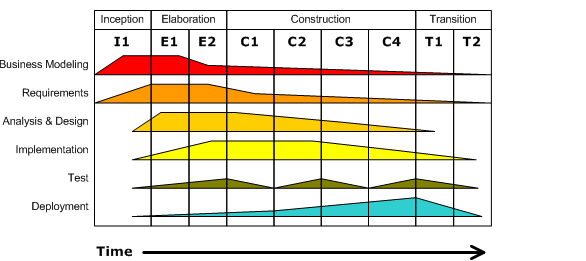
\includegraphics[width=0.6\textwidth]{image1.png}
   \caption{Exemplo de um Processo Unificado}
\end{figure}

\clearpage

\textbf{O Processo Unificado divide-se em quarto fases:}
\\

\begin{enumerate}
\item \textit{Inception} – justifica-se a execução do projeto, ou seja, tenta-se adquirir um conhecimento do que irá ser preciso para concluir o projeto e quando concluído, os resultados deste.

\item \textit{Elaboration} – conclui-se de certa forma a fase de \textit{inception}, visitando com mais detalhe todos os fatores de risco, \textit{reward} e recursos que este irá trazer. Convém ser o mais completo e detalhado possível visto que na fase seguinte vai proceder-se à construção do projecto.

\item \textit{Construction} – começa-se a construção do que irá ser uma versão operacional do projeto. O foco principal nesta fase é a construção de features discutidas anteriormente. É de valor notar que em projetos de maior dimensão esta fase poderá ter varias iterações.

\item \textit{Transition} – o foco nesta fase será transitar o projeto de um ambiente de desenvolvimento para um ambiente de produção, pondo o produto disponível ao cliente final, para que este o perceba e o use. Nesta fase faz-se o treino do cliente final e o beta testing para validar o projeto em relação às expectativas do cliente final. De seguida compara-se o estado do projeto nesta fase à fase de Inception e se tudo estiver bem, faz-se uma \textit{release}.

\end{enumerate}
%--------------------------------------------------------------------------------------------- Feito

\textbf{Vantagens do Processo Unificado:}
\begin{itemize}
\item O cliente não precisa de esperar muito tempo para entrar em contacto com um resultado prático.
\item Quando terminado o desenvolvimento do projeto é muito difícil encontrar erros dada a facilidade de os corrigir anteriormente.
\item Os riscos de grau mais elevado são trabalhados em primeiro lugar, dando assim alguma confiança no desenvolvimento do projeto
\end{itemize}

\textbf{Desvantagens do Processo Unificado:}
\begin{itemize}
\item Poderá haver desorganização em períodos mais avançados no projeto.
\item Aumento de gastos em implementações de varias versões do projetos.
\end{itemize}

%--------------------------------------------------------------------------------------------- Feito

\clearpage

\section{Gestão de Riscos}

Nesta avaliação dos riscos para o nosso projeto, identificámos que existem três grandes áreas: a de Relações Humanas, a de Tecnologia e a de Desenvolvimento do projeto.
\\
\\ 
Na categoria de RH identificámos que os principais problemas têm a haver com a relação entre membros do grupo e o comportamento de cada um.
\\
\\
Um outro facto de grande impacto que se prevê ser uma fonte de conflitos é a existência de dois gestores. Tendo já justificado esta organização de equipa incomum, os membros do projecto estão cientes que este tipo de organização pode complicar a tomada de decisões e atrasar o projecto, fazendo deste facto um risco de prioridade média.
\\
\\
Na categoria de Tecnologia identificámos que bugs e a segurança são os principais riscos a ter em conta e, iremos dar ênfase à segurança no projeto, visto que uma das partes mais criticas é o tipo de informação que iremos tratar.\\\\ Por ultimo, na categoria de desenvolvimento do projeto, identificámos que, sem surpresa, o maior problema são os atrasos que poderão acontecer, podendo estragar planos e horários planeados para a completação do projeto.\\\\ Em geral achamos que os nossos riscos irão ser de natureza comum a todos os grupos, são riscos que a maioria dos projetos, quer a nível académico ou profissional, encontram, não significando que os podemos levar menos a serio, sendo esta a causa de projetos falhados em varias áreas.

\clearpage
\subsection{Riscos de Recursos Humanos}
\begin{enumerate}
\item Má comunicação entre os elementos do grupo.
\item Falta de empenho de um ou mais elementos do grupo.
\item Falta de conhecimento em geral ou numa área especifica.
\item Baixa de um membro do grupo.
\item Falta de \textit{química} entre membros do grupo.
\item Atraso na entrega de trabalho de um membro do grupo.
\item Desistência de um membro do grupo.
\item Dois gestores
\end{enumerate}
\subsection{Riscos de Tecnologia}
\begin{enumerate}
\item [9] \textit{Spaghetti code} - a partir de um ponto mais avançado no projeto poderá haver desorganização do código efetuado.
\item [10] Código inútil proveniente de más práticas de desenvolvimento.
\item [11] Má implementação (bugs) de uma funcionalidade.
\item [12] Demora na descoberta de uma resolução para um bug encontrado na aplicação.
\item [13] Demora no \textit{patching} da aplicação quando esta sofre uma falha a nível de segurança.
\item [14] \textit{Updates} que pioram o uso ou a performance de SI.
\item [15] Nova vulnerabilidade de segurança devido a update realizado.
\item [16] Falta de segurança do projetos: intrusão externa à plataforma sem autorização, acesso indevido à base de dados, uso incorreto (inseguro) da plataforma.
\item [17] Má performance da plataforma em tempos de maior tráfego devido a má configuração.
\end{enumerate}
\subsection{Riscos no desenvolvimento do projecto}
\begin{enumerate}
\item [18] Atrasos na entrega do projeto
\item [19] Falta de funcionalidades na entrega do projeto final - Na entrega do projeto final ficamos aquém das expectativas que foram impostas no planeamento do projeto.
\item [20] Requisitos incompletos - Não identificação de todos os requisitos essenciais para o bom funcionamento da plataforma em tempo de desenvolvimento.
\end{enumerate}

\begin{table}[h]
\centering
\begin{tabular}{|l|l l l|}
\hline
Riscos                              & Tipo             & Probabilidade & Impacto \\ \hline
1				                    & Recursos Humanos & Baixa         & 2       \\ \hline
2                               	& Recursos Humanos & Média         & 2       \\ \hline
3                                	& Recursos Humanos & Média         & 3       \\ \hline
4                          			& Recursos Humanos & Baixa         & 3       \\ \hline
5             						& Recursos Humanos & Média         & 3       \\ \hline
6                            		& Recursos Humanos & Média         & 2       \\ \hline
7                     				& Recursos Humanos & Baixa         & 3       \\ \hline
7                     				& Recursos Humanos & Média         & 3       \\ \hline
8        							& Tecnologia       & Elevada       & 2       \\ \hline
9 									& Tecnologia       & Baixa         & 2       \\ \hline
10                   				& Tecnologia       & Elevada       & 2       \\ \hline
11                  				& Tecnologia       & Média		   & 2       \\ \hline
12 									& Tecnologia       & Média         & 3       \\ \hline
13                                	& Tecnologia       & Baixa         & 2       \\ \hline
14                                	& Tecnologia       & Média         & 3       \\ \hline
15                                	& Tecnologia       & Elevada       & 3       \\ \hline
16                                	& Tecnologia       & Média         & 3       \\ \hline
17                                	& Desenvolvimento  & Elevada       & 1       \\ \hline
18                                	& Desenvolvimento  & Média         & 2       \\ \hline
19                                	& Desenvolvimento  & Baixa         & 1       \\ \hline
\end{tabular}
\caption{Tabela de Riscos}
\label{riscos}
\end{table}

\subsection{RMMM}

A solução de riscos considerados elevados utilizando a RMMM segue-se abaixo.


\subsubsection{Spaghetti code}

\textbf{Mitigação:} Para não haver código desorganizado, o que pode levar a tempos excessivos de desenvolvimento, teremos de ter em mente as melhores práticas no contexto em que estamos a trabalhar, neste caso Java.\\
\\
\textbf{Monitorização:} Um elemento do grupo fazer uma inspeção periódica (a decidir mais tarde pelo manager) do código feito por outro elemento do grupo.\\
\\
\textbf{Gestão:} Caso se verifique que estamos a perder eficiência a desenvolver o projeto devido à desorganização de código, tirar um tempo só para tentar organizar o projeto.


\subsubsection{Má implementação (\textit{bugs}) de uma funcionalidade}


\textbf{Mitigação:} Tentar testar o máximo de casos possíveis relacionados com a funcionalidade em questão e ter em atenção na construção dessa mesma.\\
\\
\textbf{Monitorização:} Ter em atenção ao feedback dos utilizadores para perceber se a funcionalidade foi bem implementada.\\
\\
\textbf{Gestão:} Caso uma funcionalidade seja \textit{deployed} e esteja mal implementada, tentar perceber o que está mal o mais rápido possível para que se possa arranjar o errado. Em caso critico e, se possível, reverter a parte afetada para um estado anterior que se tenha a certeza que está correto.


\subsubsection{Falta de segurança na implementação}


\textbf{Mitigação:} Usar uma mentalidade de segurança em primeiro lugar quando na fase de desenvolvimento, visto estarmos a lidar com informação sensível e importante. Fazer um plano próprio para implementação de um sistema de segurança. Testar extensivamente.
Definir configurações de firewall (IPTables, etc...) para mitigar grande parte do risco associado.\\
\\
\textbf{Monitorização:} Ter em atenção a possíveis ataques que possam estar a ocorrer. Usar ferramentas próprias de monitorização de ataques maliciosos ao projeto (CloudFlare).\\
\\
\textbf{Gestão:} No caso de algum problema de segurança encontrado, tentar perceber a gravidade e a natureza de tal. A partir desse ponto arranjar uma solução que pareça adequada, desde um simples patch à parte afetada ao caso mais extremo, um encerramento da aplicação.


\subsubsection{Atrasos na entrega do projeto}


\textbf{Mitigação:} Ter sempre em atenção as próximas etapas de entrega. Comunicação constante entre o grupo e colaboração máxima para tentar que não exista este problema.\\
\\
\textbf{Monitorização:} Tentar perceber se nos estamos a atrasar o mais cedo possível para então se isso estiver a acontecer poder-mos ter alguma mão de manobra para arranjar solução para que não aconteça.\\
\\
\textbf{Gestão:} No caso de nos atrasar-mos numa entrega, teremos de compensar na próxima. Melhor comunicação e colaboração entre o grupo será necessário. Alocação de uma carga horária maior.


\subsubsection{Dois gestores do projecto}


\textbf{Mitigação:} Os dois membros do grupo devem sempre tomar decisões juntos, e estar abertos a alterações, para assim criar menos conflitos na gestão do projecto. Em caso de conflito, devem discutir com os restantes membros do projecto, de maneira a haver uma decisão maioritária.\\
\\
\textbf{Monitorização:} Os dois gestores devem manter-se sempre sincronizados, para as decisões serem consistentes e não haver conflito.\\
\\
\textbf{Gestão:} Em caso de conflito, os gestores devem discutir com os restantes membros do projecto, de maneira a chegarem a um consenso.

%--------------------------------------------------------------------------------------------- Refazer

\chapter{Arquitetura}

O SI vai ser dividido em quatro componentes de \textit{software} principais.

\begin{enumerate}
\item Servidor \textit{web}
\item Servidor aplicacional
\item Servidor de base de dados
\item Sistema operativo
\end{enumerate}

\noindent\textbf{1. Servidor \textit{web}}
\\
\\
O servidor \textit{web} vai processar as paginas \textit{web} para serem entregues ao cliente. As ligações vão ser protegidas com o protocolo SSL (criando paginas https). Vai ser também configurado uma \textit{firewall iptables} para limitar os ip e portos de acesso.
\\
\\
\noindent\textbf{2. Servidor aplicacional}
\\
\\
O servidor aplicacional vai servir de \textit{middleware} entre o servidor de base de dados e o servidor \textit{web}. Esta \textit{framework} vai ser programada usando o Java Applications Servers (JEE) e o \textit{WildFly}. Vai também ser auxiliada por uma API da Twilio, para autenticação de dois passos por SMS.
\\
\\
\noindent\textbf{3. Servidor de base de dados}
\\
\\
O servidor de base de dados vai instanciar uma base de dados MySQL, criada a partir do JEE.
\\
\\
\noindent\textbf{4. Sistema Operativo}
\\
\\
O Sistema Operativo escolhido para a realização do projecto foi o Ubuntu Server 14.04.
\\
\\
Estes quatro componentes de software vão ser colocados em servidores \textit{cloud}. Neste relatório vamos falar dos serviços da Amazon (AWS), mas deixamos em aberto usar outro serviço que oferecer mais vantagens ou que fique mais barato. 
\\
\\
\noindent\textbf{Amazon Web Services}
\\
\\
O servidor \textit{web} e o servidor aplicacional vão utilizar o serviço Amazon EC2 (um conjunto de servidores de computação escalável e flexível) e o servidor de base de dados vai utilizar o serviço Amazon RDS, que instância uma base de dados relacional para ser utilizada por uma aplicação \textit{web} carregada nos servidores EC2.
\\
\\
Estes serviços, devidamente configurados, vão servir de sistema distribuído para o nosso SI, assegurando todos os requisitos não funcionais, e aumentando a disponibilidade e a eficácia do SI (em comparação com usar um rede configurada na FCUL).
\\
\\
\\
Um Diagrama da interação com o cliente encontra-se no ficheiro \textit{Arquitetura.png} em anexo.


%--------------------------------------------------------------------------------------------- Feito

\chapter{Conclusão}

Perante o projecto que nos foi proposto, definimos os requisitos funcionais e não funcionais como pilares da nossa proposta de trabalho. 
Através de uma pesquisa ao \textit {website} do Portal do Utente e um conjunto de boas práticas de serviços \textit {web}, adicionamos funcionalidades possíveis de implementar no SI, e que determinam uma melhoria, tanto no serviço, como na interação com o utilizador.

%--------------------------------------------------------------------------------------------- Refazer

\begin{thebibliography}{1}

\bibitem{notes} Leslie Lamport {\em LaTEX: a document preparation system,}
  2nd edition, 1994.

\bibitem{impj} Roger S- Pressman, Bruce Maxim, {\em Software Engineering: A pratitioner's Appoach,} McGraw-Hill, 8ª edição, 1973.

\bibitem{norman} Página Web do Portal de Saúde {\em https://www.portaldasaude.pt/portal, } 2015. (Plataforma Dados Saúde)

\bibitem{fo} Página Web do Portal de Utente {\em https://servicos.min-saude.pt/utente/,} 2015. (Plataforma Dados Saúde)

\bibitem{python} Página Web sobre Python {\em https://docs.python.org/2/}, 2015. (Documentação Python 2.7).

\bibitem{java} Página Web sobre Java {\em https://docs.oracle.com/javase/8}, 2015 ( Documentação Java SE 8).

\bibitem{amazon} Amazon Web Service {\em https://aws.amazon.com/}, 2015.

\bibitem{encript} Let's Encript {\em https://letsencrypt.org/}, 2015. (Certificados SSL)

\end{thebibliography}

\end{document}

%--------------------------------------------------------------------------------------------- Refazer